\section{Interface utilisateur}
L'interface utilisateur se présentera sous la forme de plusieurs interfaces utilisateur permettant d'accéder aux différentes fonctions du programme.
On peut distinguer plusieurs grandes fonctionnalités :
\begin{itemize}
  \item Un menu principal.
  \item Le plateau et l'interface de jeu.
  \item Un menu de sauvegarde de partie depuis le jeu.
  \item Un menu de chargement de partie depuis le jeu.
  \item Un menu de chargement de partie depuis le menu.
\end{itemize} 

\subsection{Menu principal}
Il s'agit de l'interface que verra le joueur au lancement du jeu. 
Depuis ce menu, il peut créer ou charger une partie, ainsi que voir l'aide.
Les paramètres de création de partie seront obtenus avec un sous-menu de creation.
Les fonctionnalités de ce menu sont détaillées dans le diagramme de cas d'utilisation \ref{fig:useCaseMainMenu}.
\begin{figure}[h!]
    \centering
    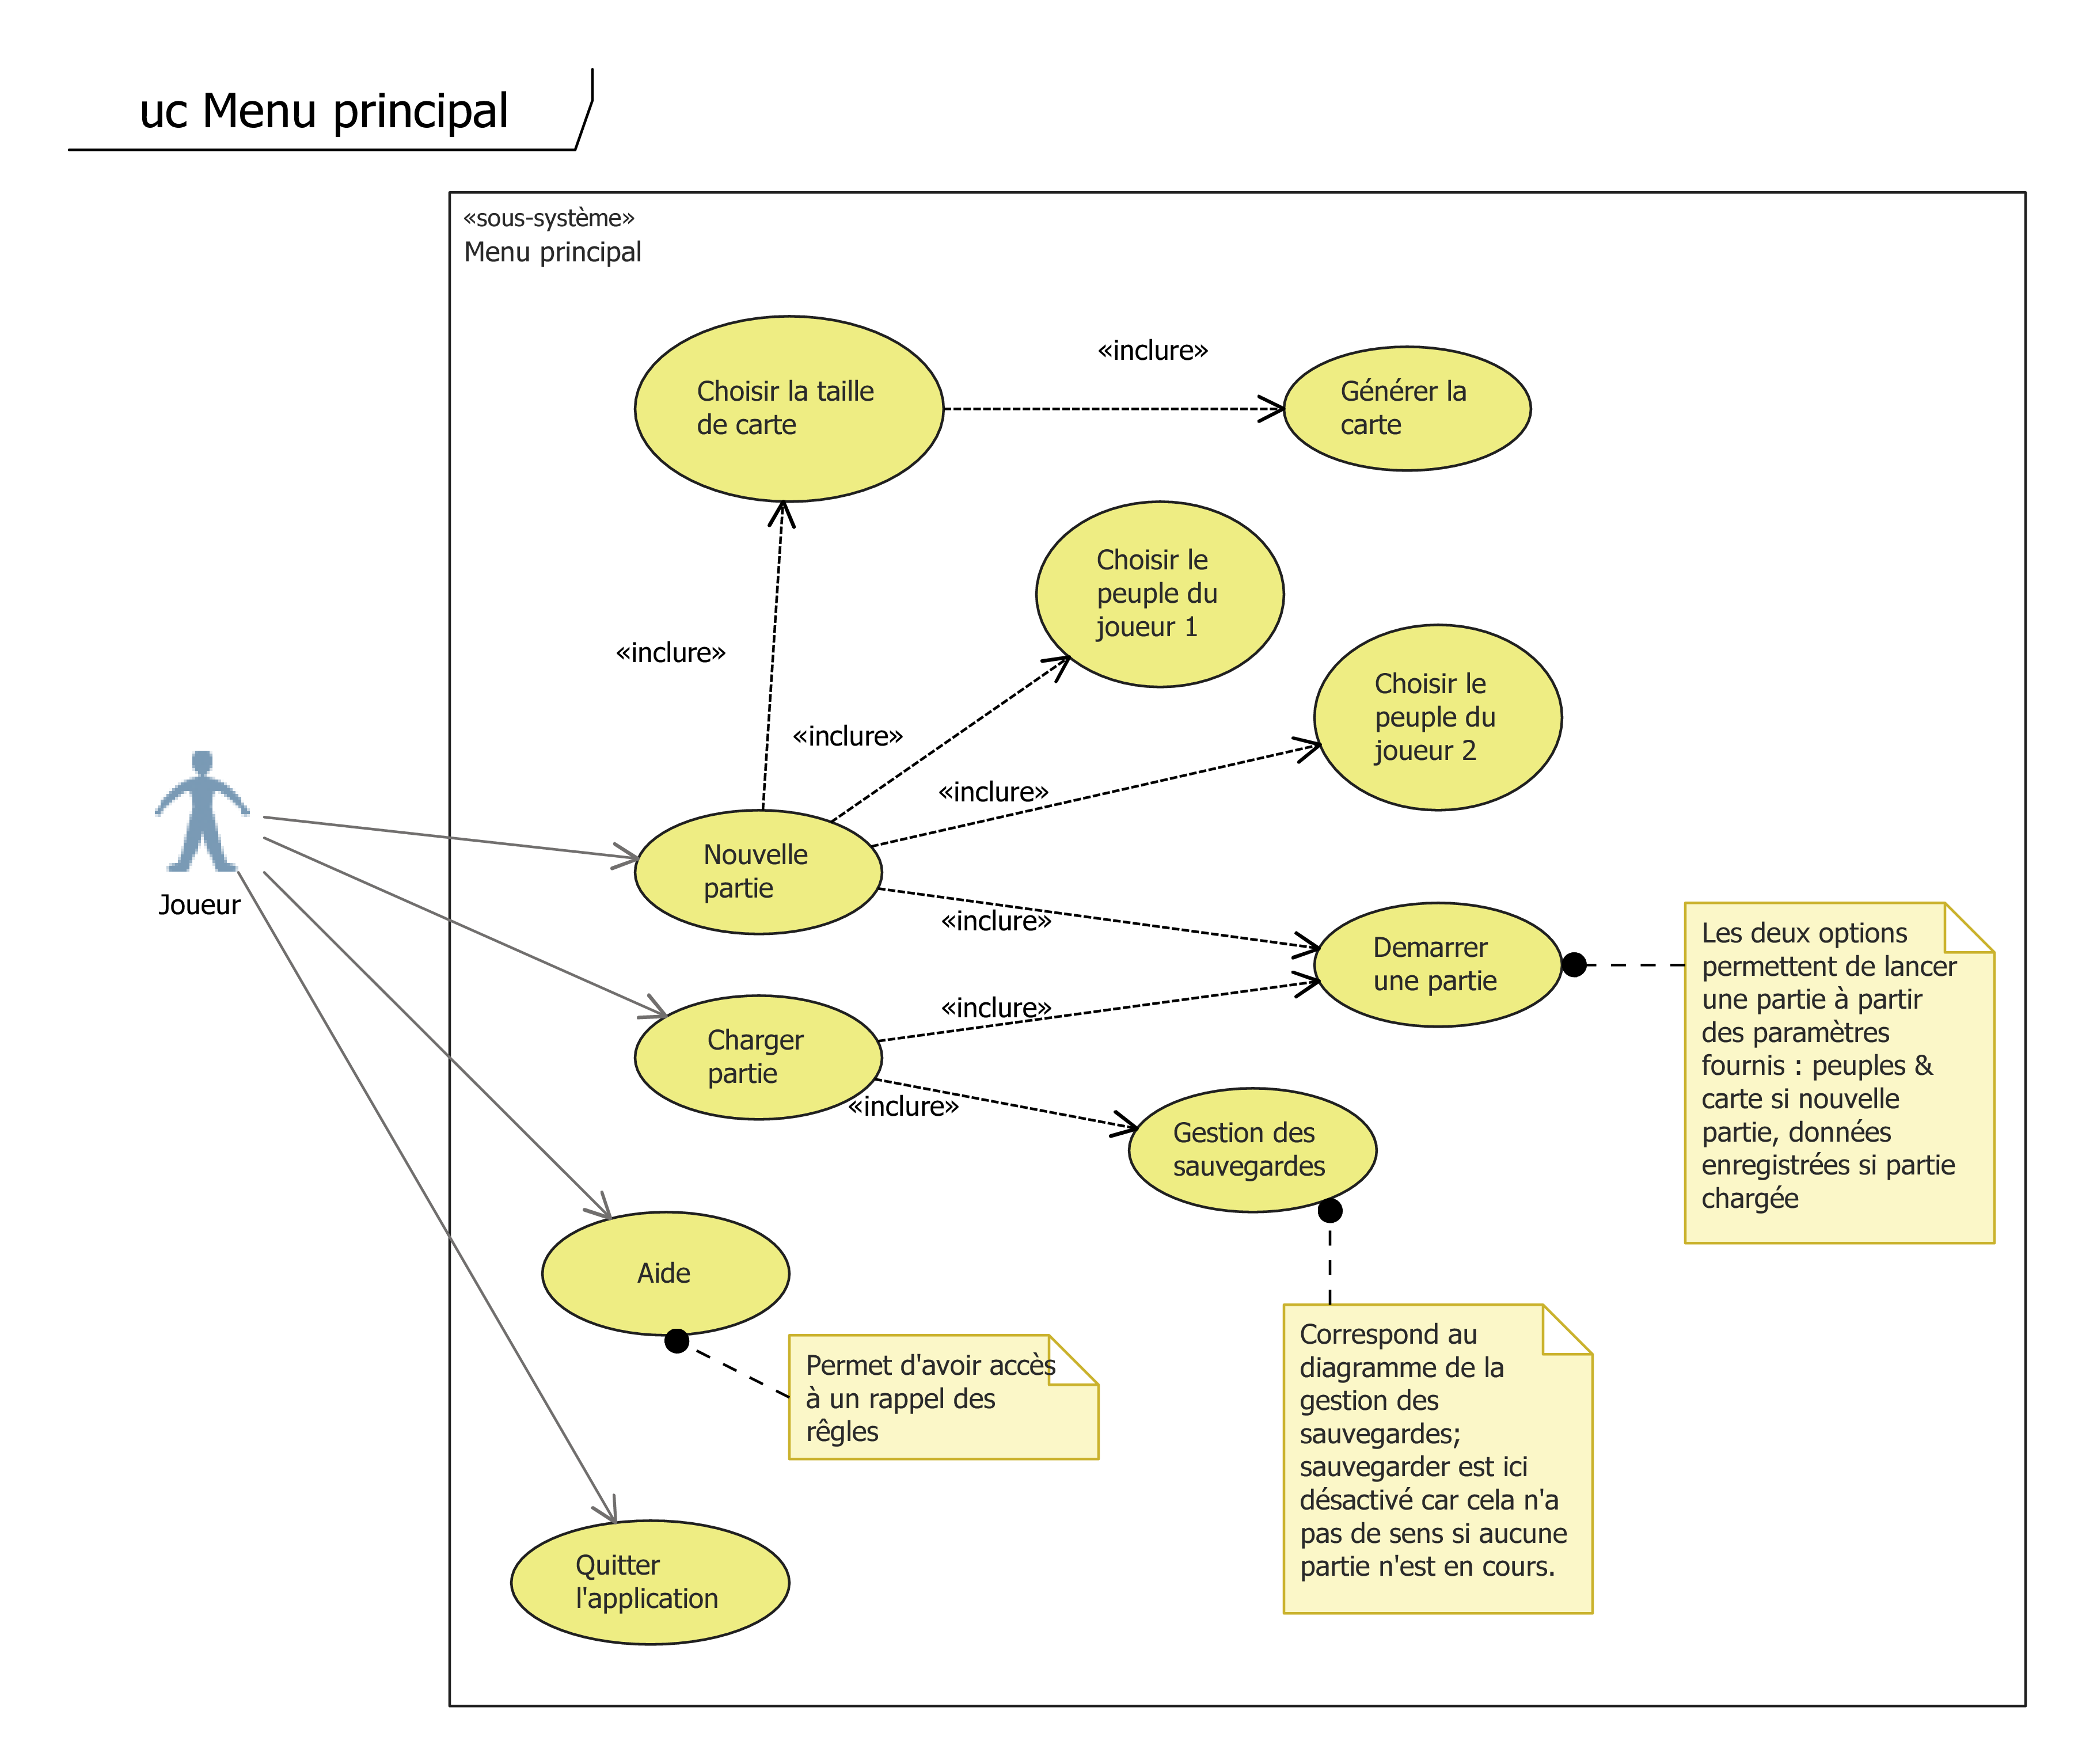
\includegraphics[width=0.8\textwidth]{res/MenuPrincipal.png}
    \caption{Fonctions du menu principal}
    \label{fig:useCaseMainMenu}
\end{figure}


\subsection{Interface durant le jeu}
L'interface utilisée au cours du jeu, dite 'In-game', représente l'interface la plus vue par le joueur. C'est donc celle qui est le plus à soigner et à perfectionner.
Plusieurs actions peuvent être réalisées par l'utilisateur depuis cette interface; celles-ci sont référencées sur le diagramme de cas d'utilisation \ref{fig:useCaseGame}.
\begin{figure}[h!]
    \centering
    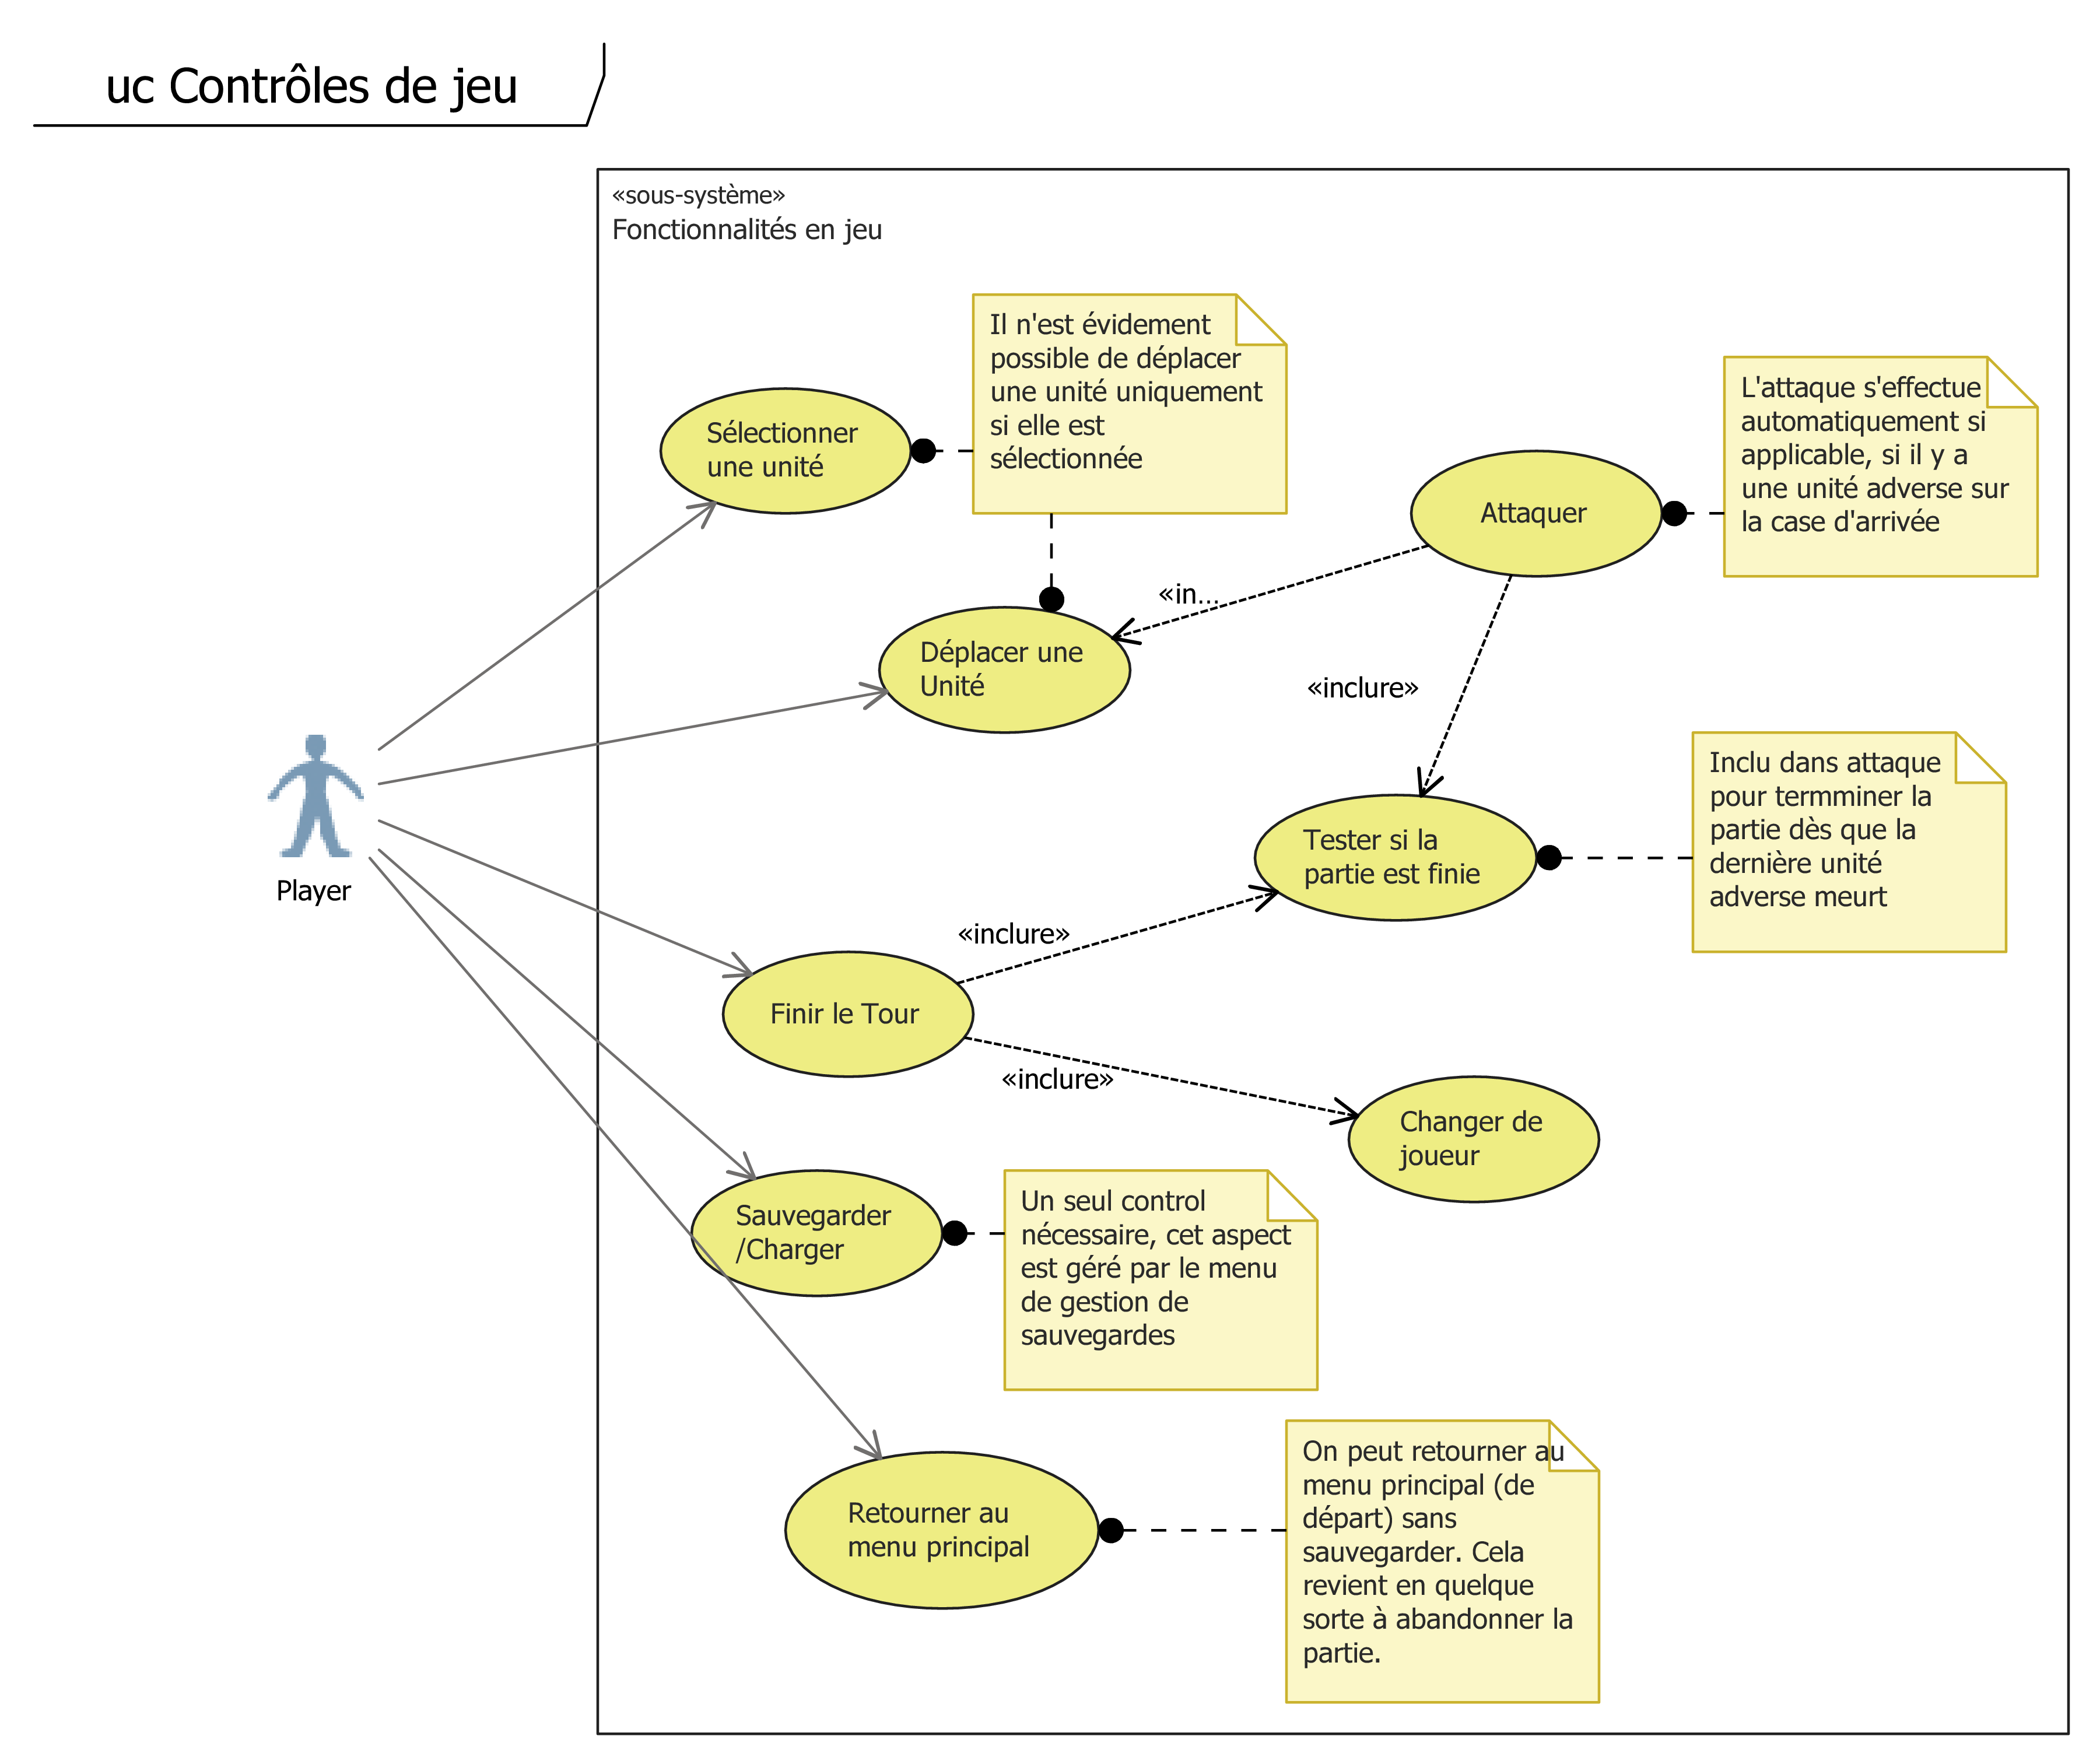
\includegraphics[width=0.8\textwidth]{res/ControleJeu.png}
    \caption{Fonctionnalités en cours de partie}
    \label{fig:useCaseGame}
\end{figure}

\subsection{Menu de gestion des sauvegardes}
Les 3 dernières fonctionnalités présentées au début de cette section sont très similaires. 
On se propose de les réunir en une seule interface.
Ce menu regroupera donc les fonctionnalités de sauvegarde et de chargement de partie, depuis le menu et le jeu. 
Lorsqu'on y accède depuis le menu principal, on grisera ou cachera l'option de sauvegarde, qui n'a pas de sens ici.
Ces fonctionnalités sont présentées dans le diagramme de cas d'utilisation \ref{fig:useCaseSaveMenu}.
\begin{figure}[h!]
    \centering
    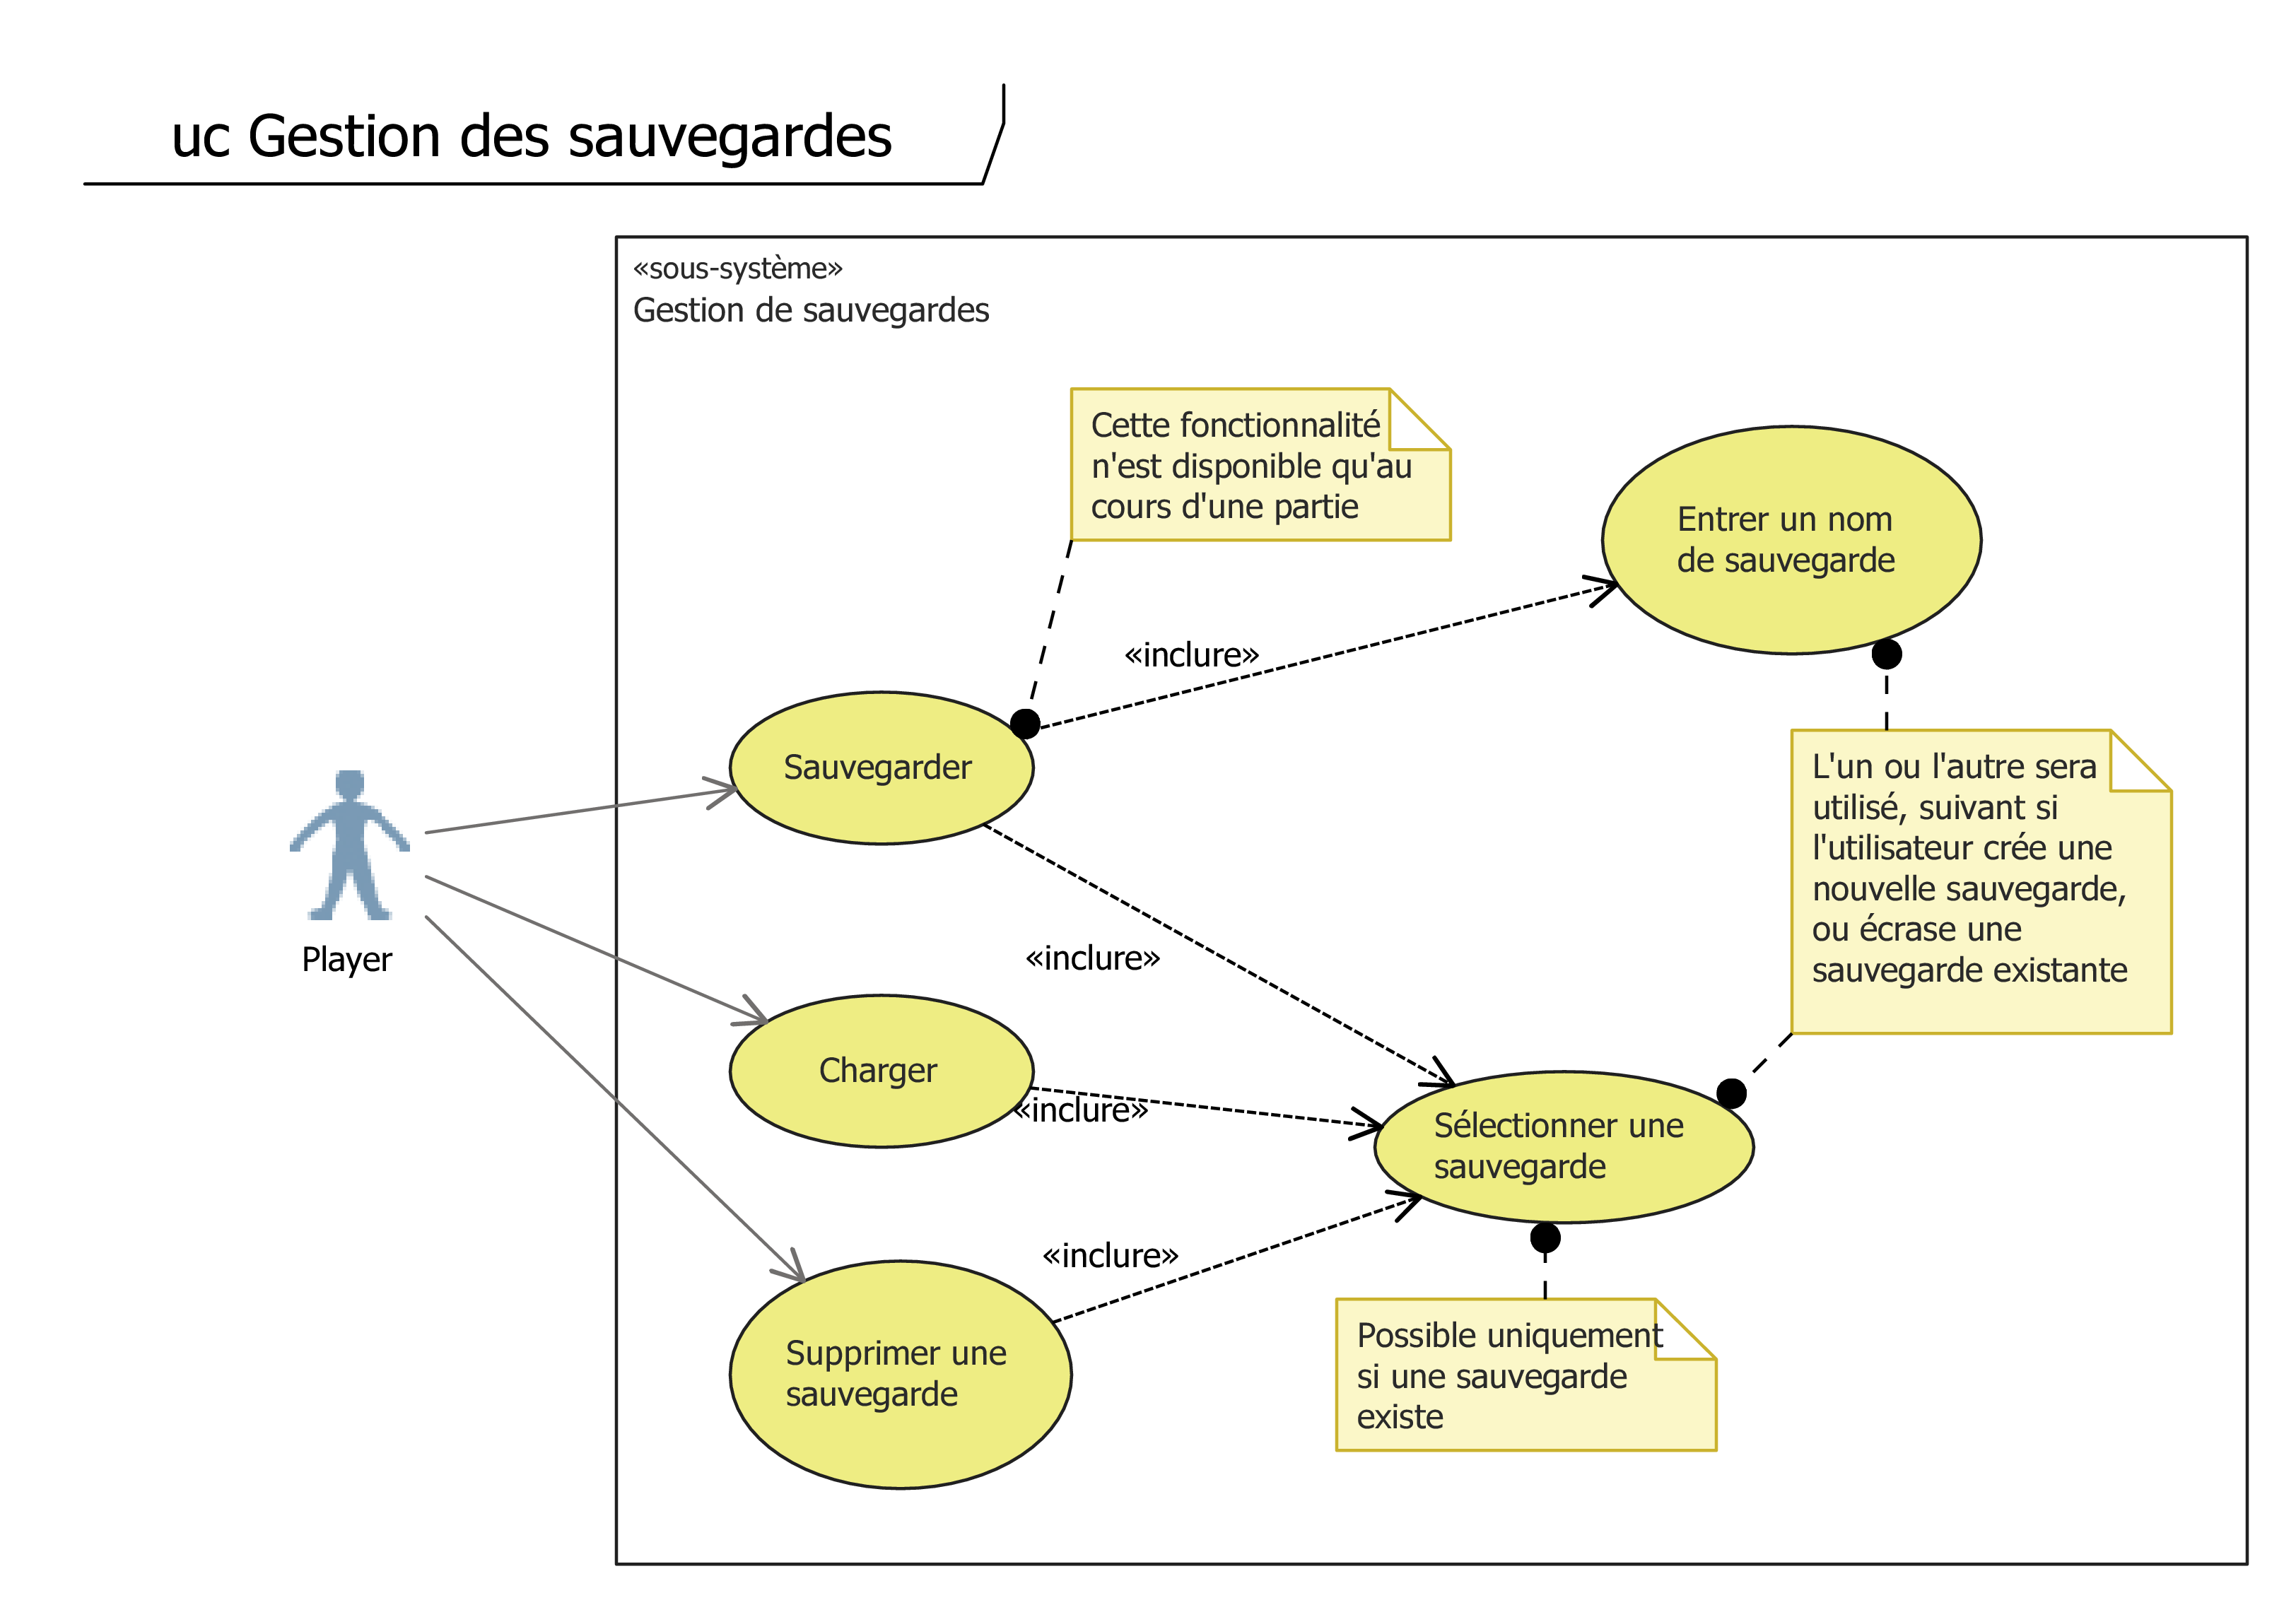
\includegraphics[width=0.8\textwidth]{res/SauvegardeMenu.png}
    \caption{Cas d'utilisation du menu de sauvegarde}
    \label{fig:useCaseSaveMenu}
\end{figure}
